The visualisations in the following two subsections manipulate matrices of scores (such as coverages or intensities) in some way, such as clustering them, or summarising them by some defined grouping. The common interface for creating matrices of scores at regular distances from a reference point, such a TSS, is the \texttt{featureScores} function. The following example samples smoothed coverages between 5000 bases upstream of gene TSSs, and 1000 bases downstream of the TSS, at 1000 base intervals, in the PrEC and LNCaP immunoprecipitated samples. The scores are then subtracted from each other.

\begin{Schunk}
\begin{Sinput}
 prostateCvgs <- featureScores(samples.list[c("PrEC IP", "LNCaP IP")], gene.anno,
                               up = 5000, down = 1000, freq = 1000, s.width = 500)
 prostateCvgs
\end{Sinput}
\begin{Soutput}
An object of class 'ScoresList'.
Tables: PrEC IP, LNCaP IP.
Features:
GRanges with 24966 ranges and 2 elementMetadata values:
          seqnames               ranges strand   |      name      symbol
             <Rle>            <IRanges>  <Rle>   | <integer> <character>
      [1]     chr1   [ 781253,  783614]      +   |   7896759   LOC643837
      [2]     chr1   [ 850983,  869824]      +   |   7896761      SAMD11
      [3]     chr1   [ 885829,  890958]      +   |   7896779      KLHL17
      [4]     chr1   [ 891739,  900345]      +   |   7896798     PLEKHN1
      [5]     chr1   [ 938709,  939782]      +   |   7896817       ISG15
      [6]     chr1   [ 945365,  981355]      +   |   7896822        AGRN
      [7]     chr1   [1092346, 1092441]      +   |   7896859         ---
      [8]     chr1   [1093105, 1093195]      +   |   7896861         ---
      [9]     chr1   [1094247, 1094330]      +   |   7896863         ---
      ...      ...                  ...    ... ...       ...         ...
  [24958]     chrY [19611913, 19614093]      -   |   8177222        CD24
  [24959]     chrY [19640262, 19640361]      -   |   8177227         ---
  [24960]     chrY [20076704, 20124427]      -   |   8177229      BCORL2
  [24961]     chrY [20326698, 20366197]      -   |   8177232     JARID1D
  [24962]     chrY [21036941, 21090502]      -   |   8177261      TTTY10
  [24963]     chrY [21954227, 21957634]      -   |   8177273         ---
  [24964]     chrY [22001970, 22008519]      -   |   8177280         ---
  [24965]     chrY [22154873, 22165940]      -   |   8177282      TTTY13
  [24966]     chrY [22852332, 22854411]      -   |   8177344       TTTY5
  ---
  seqlengths:
    chr1 chr10 chr11 chr12 chr13 chr14 ...  chr6  chr7  chr8  chr9  chrX  chrY
      NA    NA    NA    NA    NA    NA ...    NA    NA    NA    NA    NA    NA
Region: 5000 bases up to 1000 bases down.
Smoothing: 500, 500 bases.
Sampling : 1000 bases.
\end{Soutput}
\begin{Sinput}
 prostateCvgs@scores <- list(tables(prostateCvgs)[[2]] - tables(prostateCvgs)[[1]])
 names(prostateCvgs) <- "LNCaP - PrEC"
\end{Sinput}
\end{Schunk}

This object will be used in the next few visualisation functions.

\subsection{Integrative analysis of epigenetics and gene expression}
\noindent Epigenomic data is often gathered with other data, such as gene expression. It may be of interest to see the profile of epigenetic enrichment at a variety of distances from TSSs, stratified by gene expression level. The \texttt{binPlots} function is a convenient way to look at these interactions.

\begin{Schunk}
\begin{Sinput}
 binPlots(prostateCvgs, ordering = expr, ord.label = "Cancer-Normal t-stat",
          plot.type = "heatmap", n.bins = 50)
\end{Sinput}
\end{Schunk}
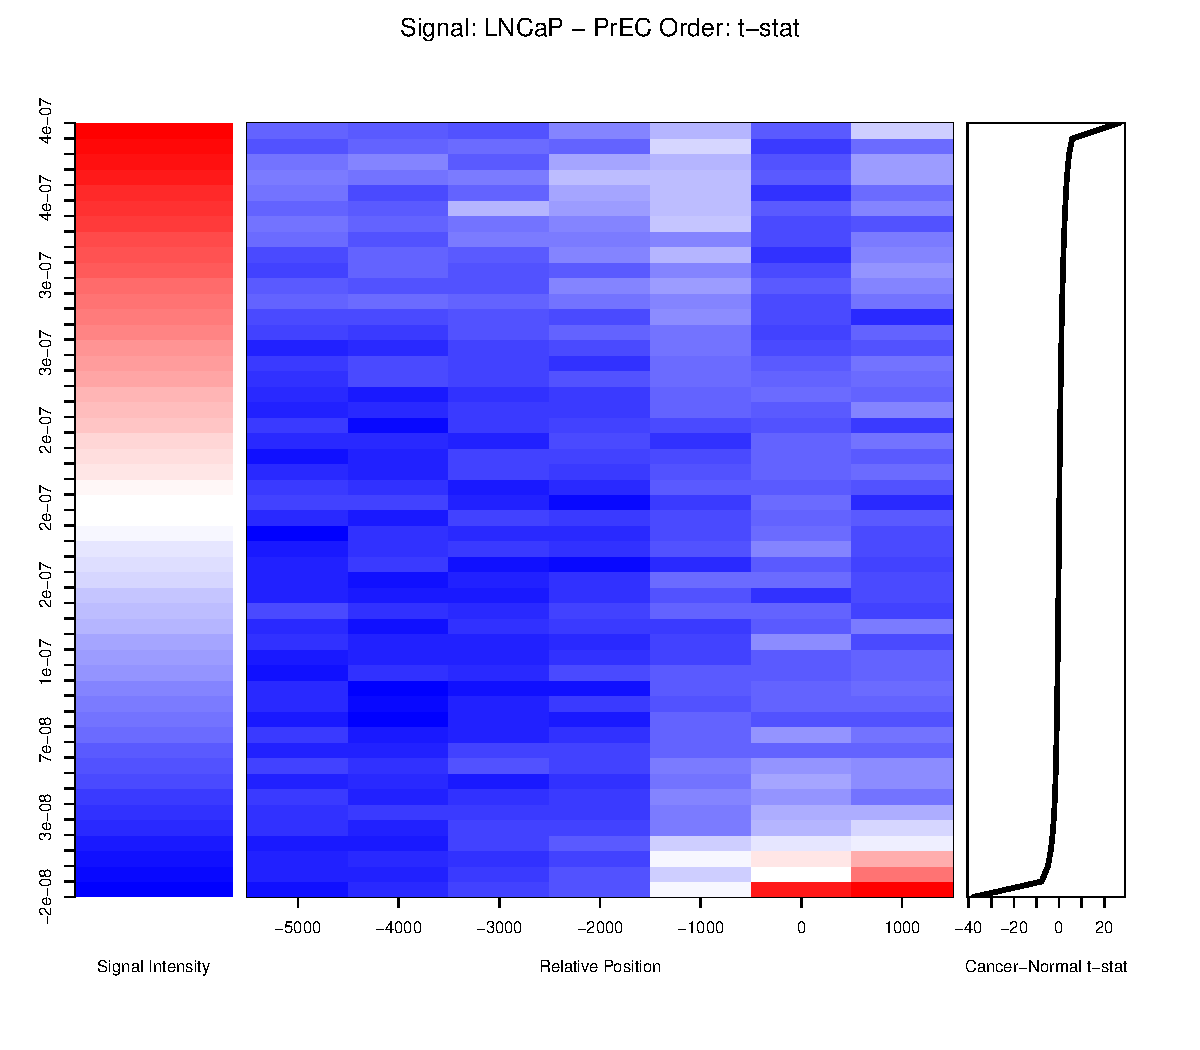
\includegraphics{visualisations-binPlotsHeatmap}

\noindent Enrichment levels (here, differential enrichment) are split into bins based on the moderated t-statistics for change in expression.  Signal for (differential) enrichment is averaged over genes in the bin and plotted as a heatmap.  As expected, the genes that are silenced in cancer exhibit higher levels of DNA methylation around their TSS, compared to normal cells.  This visualization can be represented as a lineplot, by setting \texttt{plot.type= "line"} (see below). \\

\begin{Schunk}
\begin{Sinput}
 binPlots(prostateCvgs, ordering = expr, ord.label = "Cancer-Normal t-stat",
          plot.type = "line", n.bins = 10)
\end{Sinput}
\end{Schunk}
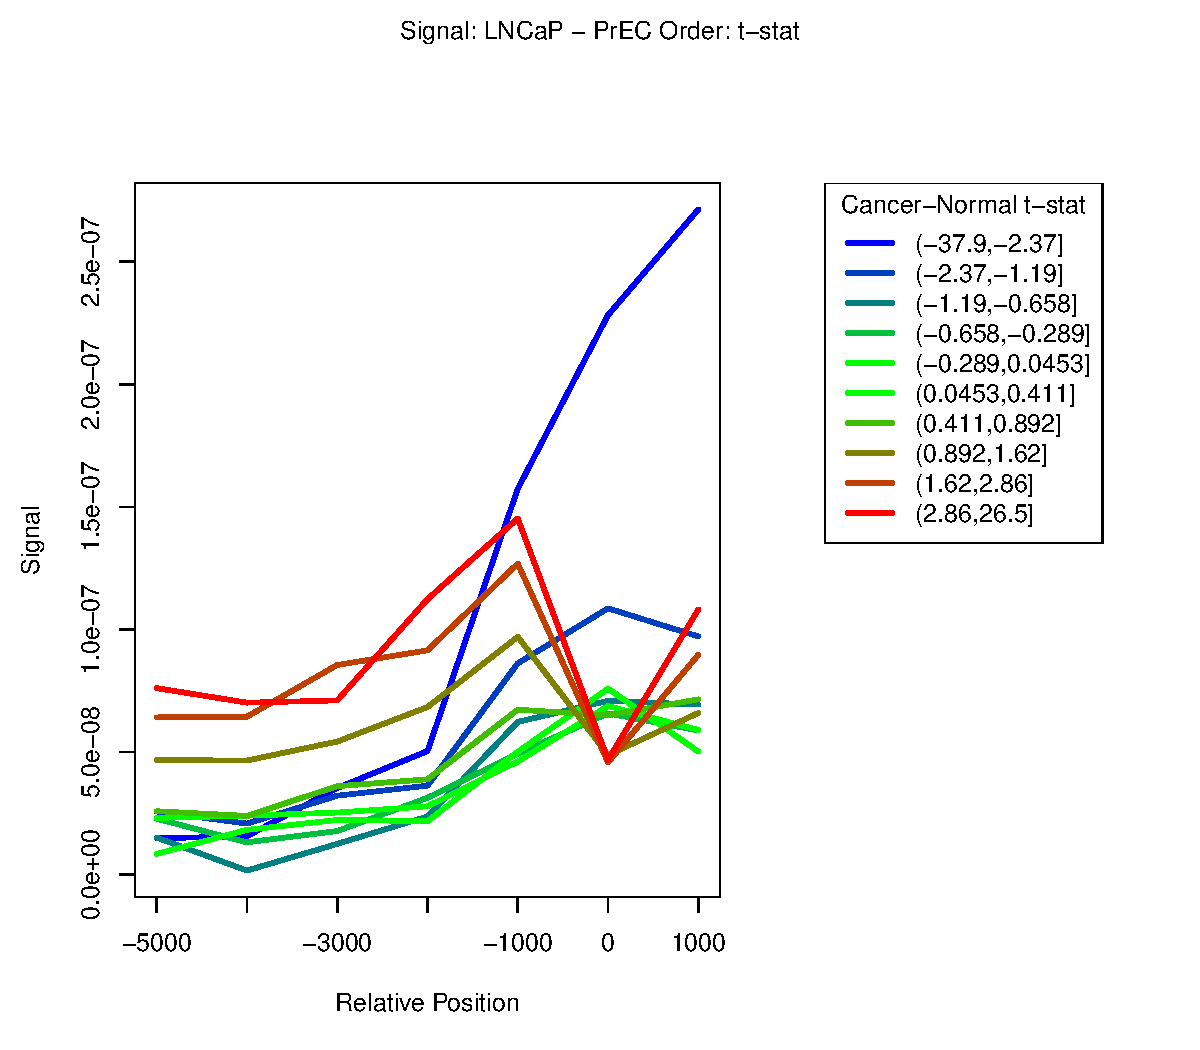
\includegraphics{visualisations-binPlotsLine}

This strategy is useful for determining the location (e.g. relative to TSS) signal most often occurs relative to expression and can be coupled to ranked gene expression levels, instead of differential expression.  These determined regions of interest relative to TSS can then be used in targeted analyses (e.g. \texttt{blocksStats}, see above).

\subsection{Gene Set Enrichment}

Sets of genes (e.g. genes disrupted in a certain type of cancer, or differentially expressed between experimental conditions) are ever-present in genomics research.  For such genes of interest, the profile of intensities or counts can be plotted versus the profile of randomly selected gene lists using the \texttt{profilePlots} function. In the following example, the DNA methylation profile of genes silenced in cancer is significantly different to random sets of genes.

\begin{Schunk}
\begin{Sinput}
 which.loss <- which(expr < -3)
 profilePlots(prostateCvgs,
              gene.lists = list(`Downregulated Genes` = which.loss),
              cols = "red")
\end{Sinput}
\end{Schunk}
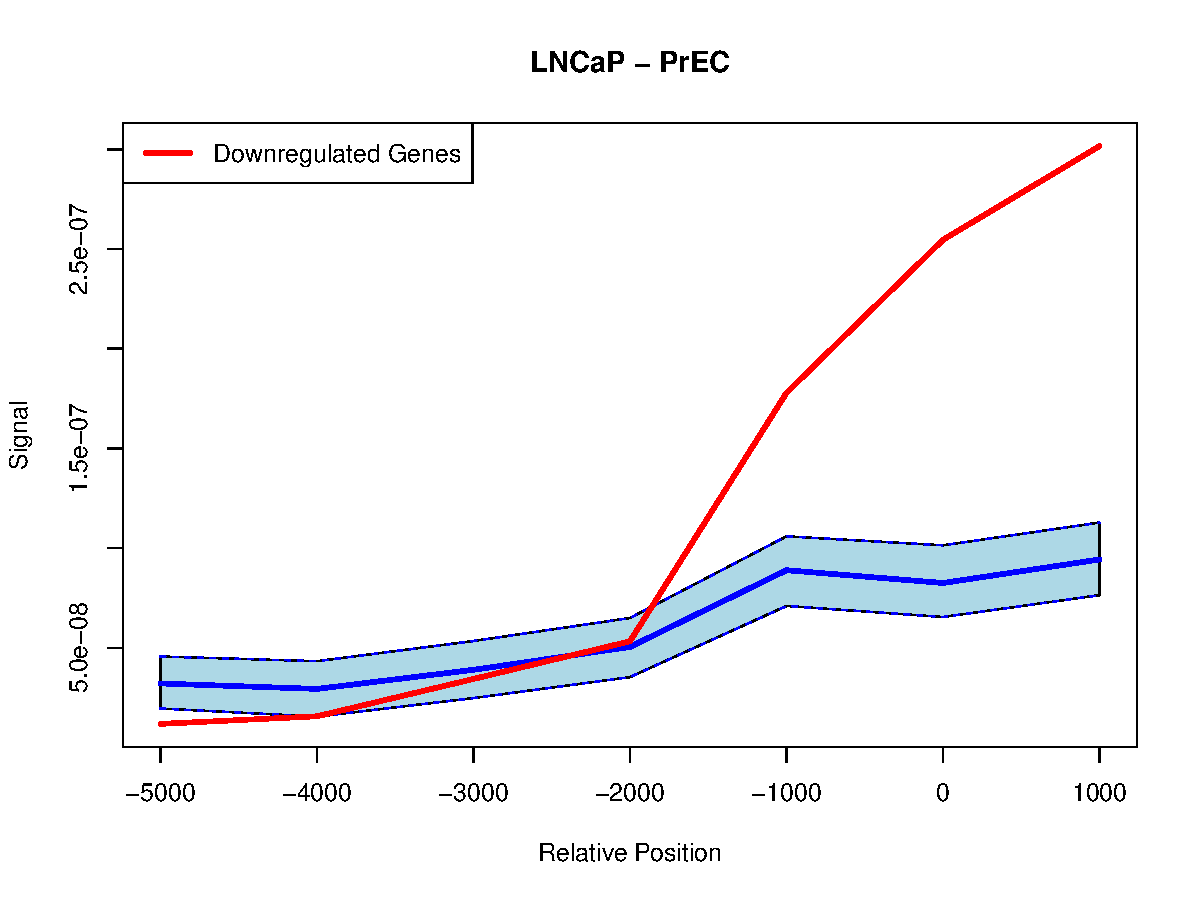
\includegraphics{visualisations-profPlots}


\noindent The blue region forms the ``null" distribution that was created by sampling random gene lists of the same size as the user-specified gene list a number of times, as set by the \texttt{nSamples} parameter. By default, the null region is a between the 0.025 and 0.975 quantiles of the null distribution. In this example, it appears that the genes silenced in cancer have a significant gain of methylation 2000 bases either side of the TSSs, in comparison to random sets of other genes.
\ \\ \ \\

\subsection{Clustering epigenomic signals}

\texttt{clusterPlots} is another way to look at read depth at regular positions around a feature (e.g. TSS). The first step is to use \texttt{featureScores} to get the coverage tables, which essentially gives a list of coverage tables for the samples used. \texttt{clusterPlots} is then called, which does k-means clustering, or if the user wants to use their own clustering algorithm, the cluster ID of each feature can be passed in. In any case, the features are grouped by their cluster memberships and plotted as either a heatmap with one row for every feature, or a set of lineplots showing the average coverage of all features belonging to each cluster. If gene expression data is also available, it can be plotted alongside the heatmaps.

\begin{Schunk}
\begin{Sinput}
 cvgs <- featureScores(H1samples[1:3], gene.anno, up = 5000, down = 2000, dist = "base",
                       freq = 200, s.width = 500)
\end{Sinput}
\end{Schunk}


\begin{Schunk}
\begin{Sinput}
 cp <- clusterPlots(cvgs, scale = function(x) sqrt(x), plot.type = "heatmap",
              t.name = "H1 Cells", n.clusters = 10)
\end{Sinput}
\end{Schunk}

\begin{Schunk}
\begin{Soutput}
null device 
          1 
\end{Soutput}
\end{Schunk}

Here, we have scaled the signal using the square root transformation.  If you don't specify this, no scaling is done.

\begin{figure}[!h]
    \begin{center}
        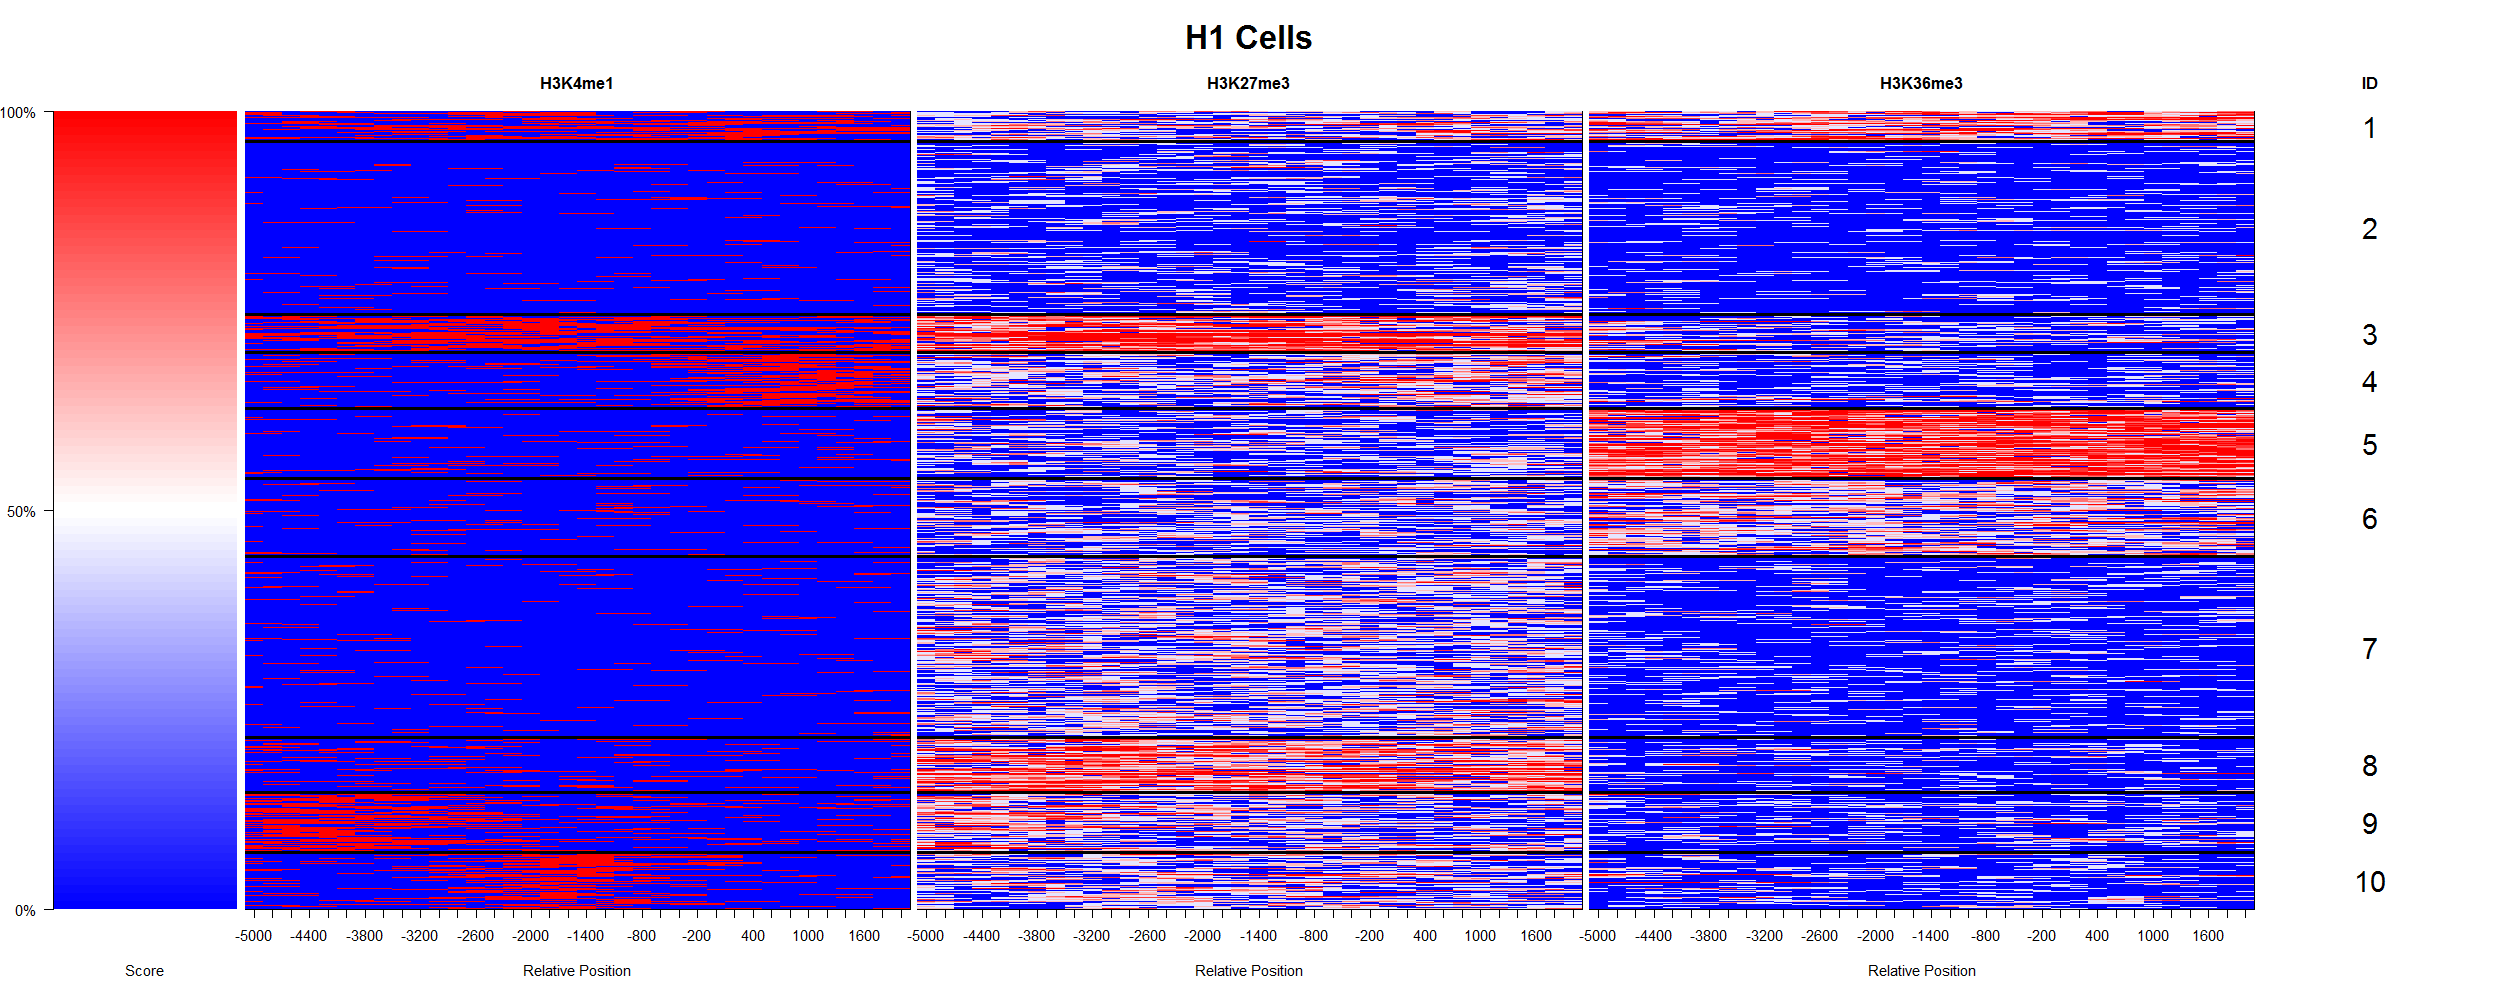
\includegraphics[height=0.48\textheight, width = 1.1\textwidth]{clusterPlot.png}
    \end{center}
\end{figure}

Note that we have saved the output of \texttt{clusterPlots} (a \texttt{ClusteredCoverageList} object), which can be plotted in alternative ways, such as line plots: 

\begin{Schunk}
\begin{Sinput}
 table(clusters(cp))
\end{Sinput}
\begin{Soutput}
   1    2    3    4    5    6    7    8    9   10 
 950 5399 1187 1770 2175 2450 5675 1698 1892 1770 
\end{Soutput}
\begin{Sinput}
 clusterPlots(cp, plot.type = "line", t.name = "H1 Cells")
\end{Sinput}
\end{Schunk}
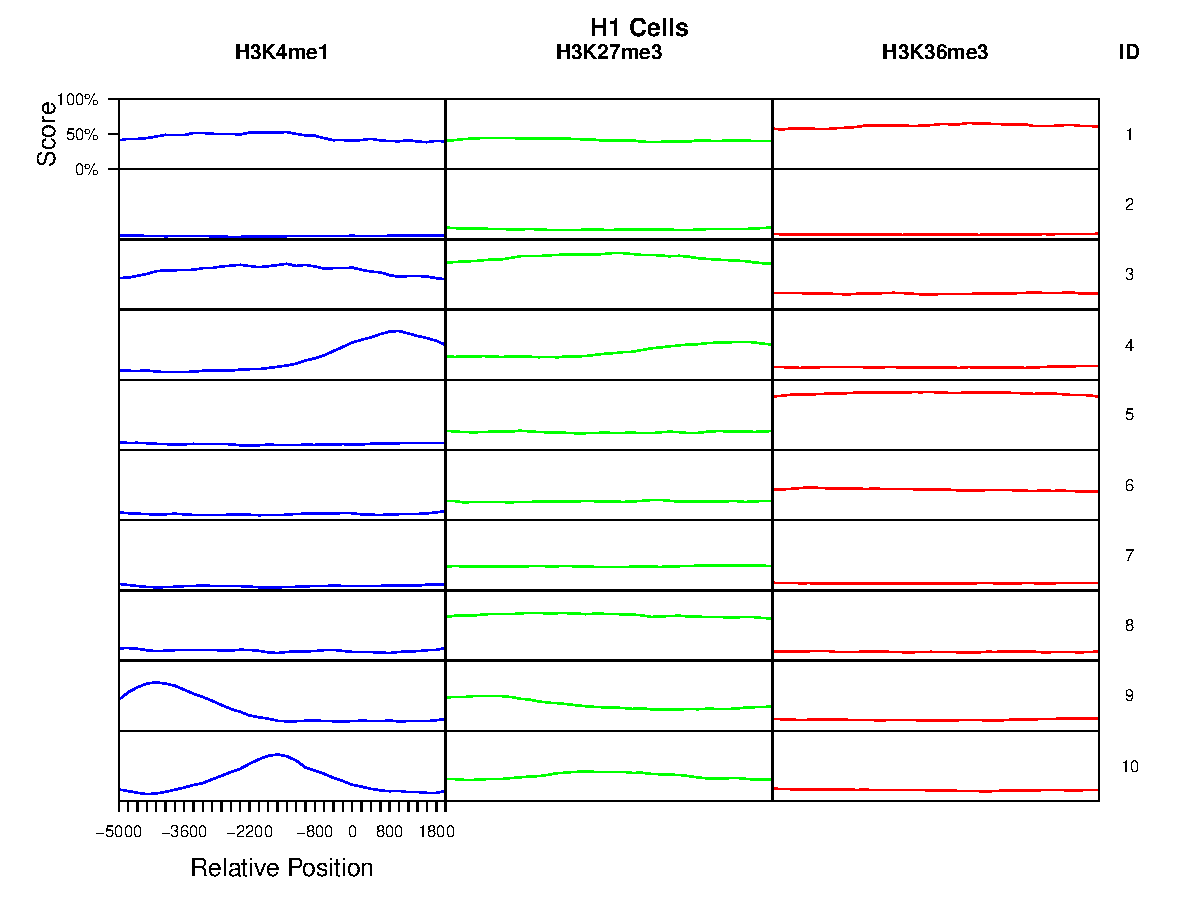
\includegraphics{visualisations-cluPlots3}

Also, this allows users to do their own clustering and use \texttt{clusterPlots} for the plotting, or to extract the cluster identifiers for downstream analyses (e.g. functional category analysis).  Furthermore, in addition to specifying a vector of expression values and plotting it alongside the clustered epigenetic signal, users can give an additional vector in the \texttt{sort.data} argument to sort on within a cluster (e.g. gene length, CpG density, etc.).
